\documentclass[a4paper,11pt, notitlepage ]{article}
\usepackage[T1]{fontenc}
\usepackage[polish]{babel}
\usepackage[utf8]{inputenc}

\usepackage{lmodern}
\usepackage{enumitem}
\usepackage{indentfirst}
\usepackage{graphicx}
\usepackage{wrapfig}
\usepackage{fancyhdr}
\usepackage{lastpage}
\usepackage{listings}
\usepackage{spverbatim}

\usepackage{listings}
\usepackage{color}

\definecolor{dkgreen}{rgb}{0,0.6,0}
\definecolor{gray}{rgb}{0.5,0.5,0.5}
\definecolor{mauve}{rgb}{0.58,0,0.82}

\lstset{frame=tb,
  language=Java,
  aboveskip=3mm,
  belowskip=3mm,
  showstringspaces=false,
  columns=flexible,
  basicstyle={\small\ttfamily},
  numbers=none,
  numberstyle=\tiny\color{gray},
  keywordstyle=\color{blue},
  commentstyle=\color{dkgreen},
  stringstyle=\color{mauve},
  breaklines=true,
  breakatwhitespace=true,
  tabsize=3
}

\usepackage{hyperref}
\hypersetup{
    colorlinks=true,
    linkcolor=black,
    filecolor=magenta,      
    urlcolor=blue,
}



\pagestyle{fancy}
\fancyhf{}
\setcounter{page}{1}
\rfoot{Strona \thepage \hspace{1pt} z \pageref{LastPage}}
\selectlanguage{polish}
\makeatletter
\newcommand{\linia}{\rule{\linewidth}{0.4mm}}
\renewcommand{\maketitle}{\begin{titlepage}
    \vspace*{1cm}
    \begin{center}\small
    Politechnika Warszawska\\
    Wydział Elektryczny
    \end{center}
    \vspace{3cm}
    \noindent\linia
    \begin{center}
      \LARGE \textsc{\@title}
         \end{center}
     \linia
    \vspace{0.5cm}
    \begin{flushright}
    \begin{minipage}{8cm}
    \textit{\small Autorzy:}\\
    \normalsize \textsc{\@author} \par
    \end{minipage}
    \end{flushright}
    \vspace*{\stretch{6}}
    \begin{center}
    \@date
    \end{center}
  \end{titlepage}%
}
\makeatother
\author{Aleksei Haidukevich, nr albumu 295233 \newline Jakub Korczakowski, nr albumu 291079 \newline Marharyta Kruk, nr albumu 295235 \newline Maciej Leszczyński, nr albumu 291085 \newline Piotr Rosa, nr albumu 291112}
\title{System do analizy sentymentów spółki na podstawie wpisów w mediach społecznościowych.}

\frenchspacing

\begin{document}
\maketitle
\setcounter{page}{2}
\tableofcontents
\newpage

\section{Etap 1 - Zbieranie danych}
\textbf{czas: 4.11.2019 - 15.12.2019}
\subsection{Opis} 
W pierwszym etapie projektu najważniejszym celem było utworzenie narzędzi do zbierania danych z Twittera i Reddita. Zostaną one użyte w celu stworzenia zbioru danych pozwalającego na naukę i testowanie algorytmów. Pobrane wiadomości i nagłówki będą składowane w bazie danych. Ten etap prac zawierał również przygotowanie infrastruktury zdolnej analizować i przechowywać zebrane dane.
\subsection{Zadania}
    \subsubsection{Analiza dostępności API mediów społecznościowych}
    Odpowiedzialni: \textbf{Piotr Rosa, Aleksei Haidukevich}\\
    Po przeanalizowaniu API zdecydowaliśmy się wykorzystać media społecznościowe \textbf{Twitter} i \textbf{Facebook}. API Twittera jest bardzo rozwinięte i pozwala na swobodny dostęp do tweetów, nawet w przypadku darmowej wersji konta. Zdecydowaliśmy się pobierać tweety wykorzystując bibliotekę Pythona - \textbf{Tweepy}. W przypadku Facebooka korzystamy z programu \textbf{FacePager}. Jest to program pozwalający pobierać wszystkie posty z wybranej strony i zapisać je do pliku z rozszerzeniem csv. Opcjonalna jest dodatkowa konwersja do JSON. Posty można pobierać z całego okresu istnienia strony.
    \subsubsection{Analiza dostępnej infrasturktury do przetwarzania danych.} 
    Odpowiedzialny: \textbf{Jakub Korczakowski}\\
    W docelowej aplikacji przetwarzającej dane w czasie rzeczywistym planujemy użyć:
    \begin{description}
        \item[Apache Hadoop] do pobierania tweetów w czasie rzeczywistym,
        \item[Apache Spark] do przetwarzania danych i uruchamiania modeli,
        \item[MS SQL] do przechowywania tweetów. 
    \end{description}

    Elementy architektury aplikacji prawdopodobnie ulegną jeszcze zmianie podczas dalszego rozwoju projektu.
    \subsubsection{Analiza i wybór sposobu wdrożenia aplikacji (rozwiązania chmurowe)} 
    Odpowiedzialni: \textbf{Jakub Korczakowski, Maciej Leszczyński}\\
    Po analizie potrzeb naszego projektu zdecydowaliśmy się wykorzystać rozwiązanie chmurowe, ponieważ pozwala one na zapewnienie dostępu do zasobów projektowych(takich jak bazy danych czy maszyny wirtualne) dla wszystkich pracujących nad projektem.
    
    Wśród dostawców infrastruktury chmurowej można wyróżnić dwie firmy, które oferują darmowe środki dla studentów. Są to Amazon (AWS) oraz Microsoft (Azure). Z powodu mniejszych możliwości oraz mniejszej ilości środków dostępnych na patformie AWS zdecydowaliśmy się wybrać platformę Azure.
    
    W obrębie tej platformy oprócz klasycznych maszyn wirtualnych dostępne są rozwiązania docelowe przeznaczone do przetwarzania dużych ilości danych, należą do nich:
    \begin{itemize}
        \item HDInsight,
        \item Azure Databricks,
        \item Azure Data Lake Services.
    \end{itemize}
    
    Pomimo tego, że te usługi znacznie ułatwają budowę projektów nie zdecydowaliśmy się na ich użycie ze względu na wysoką cenę. Planujemy używać maszyn wirtualnych i za pomocą Dockera, a w przyszłości Kubertenesa zbudować infrastrukturę projektu.
    \subsubsection{Wybór odpowiedniej bazy do składowanych danych (porównanie SQL i noSQL)} 
    Odpowiedzialni: \textbf{Jakub Korczakowski, Maciej Leszczyński}\\
    Do składowania historycznych danych w naszym projekcie będziemy wykorzystywać bazę SQL ze względu na szybkość dostępu do danych.
    \subsubsection{Stworzenie programu pobierającego dane z Twittera}
    Odpowiedzialny: \textbf{Piotr Rosa}\\
    Korzystając z biblioteki \textbf{Tweepy} udało nam się stworzyć skrypt pobierający wpisy z Twittera dotyczące wybranego słowa kluczowego. API Twittera pozwala na pobieranie naprawdę wielu szczegółów dotyczących wpisów, jednak do naszych celów nie potrzebujemy ich wszystkich. Zdecydowaliśmy się na pobieranie: ID tweeta, datę jego stworzenia, nazwę użytkownika oraz zawartość tweeta.\\
    Pobrane dane przechowujemy w tabelach, osobno dla każdej firmy, z dodatkową kolumną Sentyment, która mówi o tym, czy przesłanie wiadomości jest negatywne, czy pozytywne.\\
    Skrypt ten pobiera dane w interwałach czasowych, przy czym nie wszystkie tweety są zapisywane, a losowana jest jedynie część z nich. Wynika to z faktu, że często pojawia się więcej wpisów niż się spodziewaliśmy, a możemy nie poradzić sobie ze zbyt dużym zbiorem danych.
    \subsubsection{Stworzenie programu pobierającego dane z Facebooka}
    Odpowiedzialny: \textbf{Aleksei Haidukevich}\\
    Pobieranie danych z Facebooka przy użyciu programu FacePager pozwala na dostęp do danych niezależnie od dat powstania postów. Dzięki temu, uruchamiając program co określony czas dla wybranych stron, otrzymujemy pliki csv, z których dane przetwarzane są przy użyciu języka Python. Interesujące nas dane są analogiczne do tych w przypadku Twittera.
    \subsubsection{Instalacja wybranej bazy}
    Odpowiedzialny: \textbf{Jakub Korczakowski}\\
    Pobrane tweety składujemy w bazie SQL znajdującej się na platformie Azure. Obecnie bazy danych pomieścić może do 2GB danych, jednak w przypadku gdy potrzebne nam będzie więcej przestrzeni możemy w każdej chwili zwiększyć pojemność bazy. Jest to jedna z zalet użycia chmury. Baza danych dostępna jest pod statycznym adresem IP, więc jest łatwo dostępna dla każdego. Konieczne jest jedynie dostosowanie zapory sieciowej w celu umożliwienia dostępu.
    \subsubsection{Połączenie bazy danych z programami pobierającymi dane}
    Odpowiedzialny: \textbf{Jakub Korczakowski}\\
    Serwer bazodanowy działa na platformie \textbf{Azure}. Zarówno dla danych z Twittera, jak i z Facebooka, łączenie z serwerem odbywa się przy wykorzystaniu biblioteki \textbf{pyodbc}. Serwer bazodanowy na Azure posiada statyczny adres, dlatego łączenie się z nią nie jest skomplikowane. W konfiguracji połączenie trzeba podać odpowiedni login, hasło, nazwę bazy danych oraz nazwę sterownika w naszym systemie, który zostanie wykorzystany do tego połączenia. Zazwyczaj sterownik ten jest już zainstalowany, wystarczy jedynie odnaleźć jego nazwę.
    \subsubsection{Pobranie danych do bazy danych}
    Odpowiedzialny: \textbf{Maciej Leszczyński}\\
    Baza danych z której korzystamy jest bazą SQL-ową. Po nawiązaniu połączenia, polecenia wykonywane są jak w przypadku korzystania z bazy danych lokalnie. Dane będą zapisywane w bazie danych w czasie rzeczywistym za pomocą opracowanych programów.
    \subsubsection{Analiza dostępnych zbiorów opisanych klasami, pozwalających na testowanie algorytmu} 
    Odpowiedzialna: \textbf{Marharyta Kruk}\\
    Znaleziony został zbiór pozwalający na trenowanie oraz testowanie algorytmu. Zbiór zawiera 1600000 opisanych tweetów. Dla każdego tweetu został obliczony sentyment. 
    
    Zbiór znajduje się pod adresem: \href{https://www.kaggle.com/kazanova/sentiment140}{adres}.
    

\subsection{Wykonanie zadań z pierwszego kamienia milowego}
Podczas tego etapu nie byliśmy w stanie wykonać wszystkich zadań, które założyliśmy w statucie projektu. Udało nam się rozpocząć budowę modelu oraz znaleźć odpowiedni zbiór treningowy, pozwalający na analizę sentymentu. Udało się nam również poznać API Twittera oraz rozpocząć pracę nad programami pobierającymi dane. Próba wykorzystania wiadomości z Reddita zakończyła się niepowodzeniem ze względu na brak odpowiednich danych w serwisie. Trudniejsze niż przewidywaliśmy okazało się również zbudowanie klastra na platformie MS Azure. Potrzebowaliśmy więcej czasu, aby zapoznać się z możliwościami platformy, co spowodowało przesunięcie się pracy.

\section{Etap 2 - Przetwarzanie danych}
\textbf{czas: 7.01.2020 - 31.03.2020}
\subsection{Opis} 
W drugim etapie do najważniejszych celów należą cele niezrealizowane poprawnie w pierwszym etapie, czyli budowa infrastruktury do przetwarzania danych oraz stworzenie programów pobierających dane. Kolejnymi celami będzie stworzenie programów przetwarzających dane i uruchomienie modeli na przygotowanej infrastrukturze. W odniesieniu do pierwszego etapu dokonaliśmy zmiany bazy danych na bazę NoSQL, zdecydowaliśmy się wybrać bazę MongoDB.
\subsection{Zadania}
    \subsubsection{Budowa infrastruktury do przetwarzania danych}
    Odpowiedzialny: \textbf{Jakub Korczakowski}\\
    \begin{figure}[h]
        \centering
        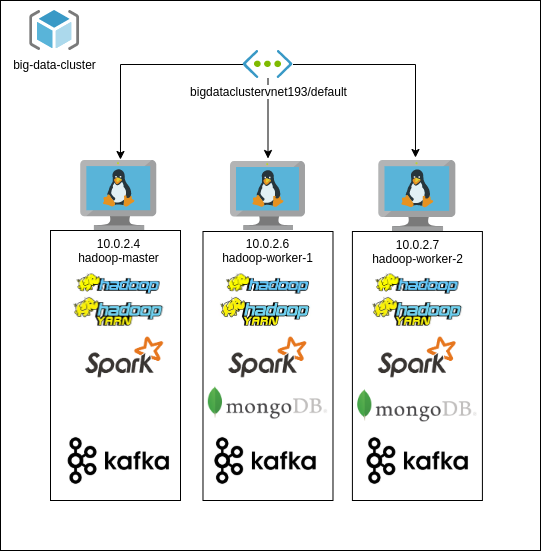
\includegraphics[width=1 \textwidth]{diagram1.png}
        \caption{Diagram przygotowanej infrastruktury.}
        \label{fig:diagram}
    \end{figure}

    W celu utworzenia infrastruktury zdolnej przetwarzać dane zostały utworzone 3 maszyny wirtualne w grupie zasobów \textbf{big-data-cluster
    } na platformie \textbf{Azure} w regionie \textbf{North Europe}. Są to odpowiednio:
    \begin{description}
        \item[hadoop-master] Standard D2s v3 (2 vcpus, 8 GiB memory),
        \item[hadoop-worker-1] Standard B2s (2 vcpus, 4 GiB memory),
        \item[hadoop-worker-2] Standard B2s (2 vcpus, 4 GiB memory). 
    \end{description}

    Ze względu na specyfikę platformy \textbf{Azure} wielkość i rodzaj maszyn może zostać przeskalowany w razie potrzeb. Wszystkie maszyny są dostępne pod publicznymi adresami IP poprzez protokół ssh. Dodatkowo maszyna \textbf{hadoop-master} posiada środowisko graficzne i można dostać się do niej również poprzez protokół RDP na porcie 3389.

    Ilość maszyn jest zdeterminowana częściowo poprzez limit nałożony na subskrypcję studencką. Limit wynosi 6 vcpus na strefę regionalną maszyn.

    \subsubsection{Instalacja narzędzi do przetwarzania danych}
    Odpowiedzialny: \textbf{Jakub Korczakowski}\\
    \begin{description}
        \item[Apache Hadoop] Został zainstalowany na klastrze. Wartość replikacji plików została zmieniona na \textbf{2} ze względu na ilość dostępnych DataNode.
        \item[YARN] Został skonfigurowany w klastrze.
        \item[Apache Spark]  Został zainstalowany na klastrze oraz skonfigurowany w trybach działania \textbf{standalone} oraz poprzez  \textbf{YARN}. Został połączony ze środowiskiem \textbf{Hadoop}.
        \item[MongoDB] Baza została zainstalowana na maszynie \textbf{hadoop-master}. Została skonfigurowana w sposób umożliwiający odwołanie się do niej z sieci lokalnej(poprzez ip \textbf{10.0.2.4}). Poprzez odpowiednie opcje konfiguracyjne możliwe jest połączenie z \textbf{Apache Spark}.
        \item[Apache Kafka] Broker Apache Kafka został zainstalowany jako klaster na wszystkich maszynach. Dodatkowo został zainstalowany Apache Zookeeper, który nadzoruje działanie brokera. 
    \end{description}   
    
    \textbf{Rola maszyn w systemach.}

    \begin{tabular}{|l|l|l|l|} \hline
        & Apache Hadoop & YARN & Apache Spark \\ \hline \hline
        hadoop-master & NameNode & ResourceManager & Master\\ \hline
        hadoop-worker-1 & DataNode & NodeManager & Slave\\ \hline
        hadoop-worker-2 & DataNode & NodeManager & Slave\\ \hline
    \end{tabular}

    \subsubsection{Baza Danych} 
    Odpowiedzialny: \textbf{Jakub Korczakowski} \\
    Baza danych została zainstalowana na maszynach \textbf{hadoop-woker-1} oraz \textbf{hadoop-woker-2}. Pierwsza z maszyn odpowiada za Twittera, a druga za Facebooka.

    \subsubsection{Potok przetwarzania danych w projekcie} 
    Odpowiedzialny: \textbf{Jakub Korczakowski} \\
    Podczas tego etapu udało nam się również zaplanować dokładniej potok przetwarzania danych w naszym projekcie. Planowany potok widoczny jest na poniższym rysunku.

    \begin{figure}[h]
        \centering
        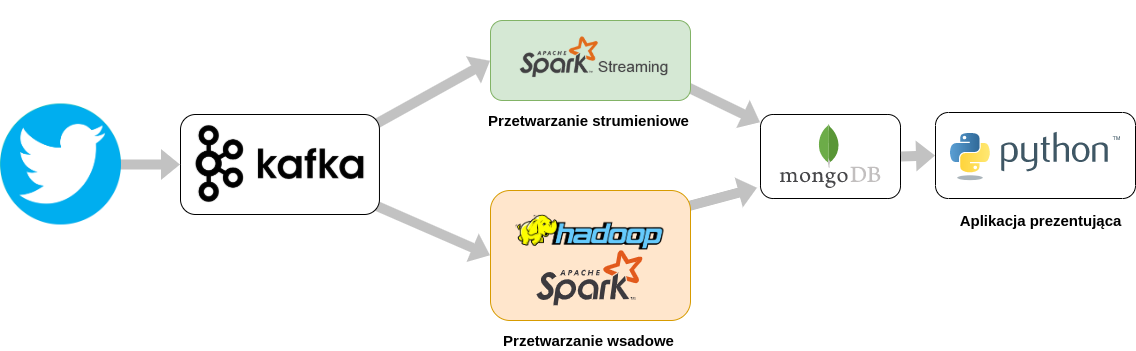
\includegraphics[width=1 \textwidth]{FlowChart.png}
        \caption{Diagram potoku danych w projekcie.}
        \label{fig:diagram}
    \end{figure}

    Do pobierania danych w czasie rzeczywistym w naszym projekcie użyjemy Apache Kafka, który za pomocą skryptów napisanych w języku Python łączył się z Twitter API i pobierał dane. Przetwarzanie strumieniowe planujemy przeprowadzić za pomocą Apache Spark Streaming, a wyniki analiz zapisać w MongoDB. Przetwarzanie strumieniowe będzie obejmować głównie analizę sentymentu pobieranych tweetów. Wyniki z bazy będą na końcu prezentowane przez napisaną przez nas aplikację.

    \subsubsection{Udoskonalenie programu do pobierania danych z Twittera} 
    Odpowiedzialny: \textbf{Piotr Rosa} \\
    Program pobierający dane działa w języku Python z wykorzystaniem biblioteki Tweepy. Pobrane dane zapisywane są z wykorzystaniem systemu Avro. Pliki zapisane w tym formacie mają strukturę podobną, umożliwiającą łatwe przekształcenie, do formatu JSON. Główną wadą zapisu danych w JSON jest fakt, że nazwy pól zapisywane są dla każdego rekordu, co znacznie zwiększa zużycie pamięci, przez co nie nadaje się on dla dużych zbiorów danych. W przypadku Avro, schemat definiujący każdy rekord, zapisany jest jeden raz dla każdego pliku. Aby umożliwić współpracę programu z platformą Hadoop, tzn. zapis zebranych plików z danymi do systemu plików HDFS, wykorzystujemy bibliotekę Pythona hdfs, a zapis plików w formacie Avro umożliwia pakiet z tej biblioteki hdfs.ext.avro.
    Program, ze względu na brak możliwości nieustannego działania maszyn, uruchamiany jest domyślnie co dwa dni. Początkowo planowaliśmy pobieranie danych w odstępach tygodniowych, ponieważ Twitter pozwala na pobranie danych historycznych z okresu tygodnia, jednak istnieją również limity zapytań. Limit ten to 1800 zapytań w ciągu 15 minut, przy czym każde zapytanie zwraca maksymalnie 100 tweetów. Nie wystarcza to do naszych celów i konieczne byłoby czekanie około godziny na pobranie wszystkich interesujących nas wpisów, dlatego zdecydowaliśmy się pobierać je częściej. Dane zapisywane są w HDFS w strukturze: \texttt{data/<nazwa\_firmy>/<nazwa\_firmy>\#.avro}, gdzie \texttt{\#} oznacza kolejny numer pobrania. Program wykorzystuje pomocniczy plik, w którym zapisywana jest liczba dotychczas wykonanych pobrań danych, zdefiniowane są nazwy firm, które śledzimy oraz numer ID ostatniego tweeta dla każdej z nich, na podstawie którego określamy jak długo pobierać tweety, aby ich nie duplikować. Wybraliśmy osiem firm, kurierskich oraz dostarczających żywność, które będziemy śledzić.

    Kroki przy tworzeniu programu:
    Na maszynie, którą posłużymy się do pobierania danych zainstalowaliśmy potrzebne biblioteki Pythona:

    \begin{verbatim}
    pip install tweepy
    pip install hdfs[avro]
    \end{verbatim}
    Następnie stworzyliśmy plik konfiguracyjny ~/.hdfscli.cfg, potrzebny do łączenia się z HDFS.
    Później został stworzony testowy program zapisujący dane do pliku w formacie .avro do HDFS oraz program odczytujący ten plik. Po uruchomieniu programu zapisującego plik, sprawdziliśmy zawartość HDFS.
    Wykonaliśmy kolejno polecenia:
    hdfscli --alias=dev
    CLIENT.list('test/')
    CLIENT.status('test/testfile.avro')

    Oto ich wyniki:
    \begin{verbatim}
    stud@hadoop-worker-1:~/scripts/tests$ hdfscli --alias=dev

    Welcome to the interactive HDFS python shell.
    The HDFS client is available as CLIENT.

    CLIENT.list('test/')
    [u'testfile.avro']
    CLIENT.status('test/testfile.avro')
    {u'group': u'supergroup', u'permission': u'644', 
    u'blockSize': 134217728, u'accessTime': 1586095573925, 
    u'pathSuffix': u'', u'modificationTime': 1586095574082, 
    u'replication': 2, u'length': 283, u'childrenNum': 0, 
    u'owner': u'stud', u'storagePolicy': 0, u'type': u'FILE', 
    u'fileId': 16815}
    Oraz wynik programu odczytującego ten plik z HDFS:
    {u'username': u'user1', u'value': 1, u'title': u'test1'}
    {u'username': u'user2', u'value': 2, u'title': u'test2'}
    \end{verbatim}

    Jak widać plik został poprawnie zapisany, istnieje możliwość odczytania go oraz widać, że został on zduplikowany.
    Gdy wszystko działało poprawnie stworzyliśmy właściwy program.

    Obserwowane firmy to: DHL, Uber Eats, FedEx, Grubhub, DoorDash, Postmates, Woolworths.

    \subsubsection{Stworzenie modelu do analizy sentymentów} 
    Odpowiedzialna: \textbf{Marharyta Kruk} \\

    Model został stworzony na zbiorze Twitter Sentiments, zawierającym 1.6 milion tweetów o \textit{niegatywnych}, \textit{pozytywnych} oraz \textit{neutralnych} sentymentach. Model do analizy sentymentów Reddita nie został stworzony z powodu trudności zebrania niezbędnych danych. Model, nauczony na zbiorze tweetow, został przyznany jako przygodny do analizy dowolnych zdań.
    Zbiór danych został początkowo przetworzony, zostały wyrzucony stop listy, zostawione stemmery.
    Wejsciem do sieci służa przetworzone słowa, każde słowo jest przedstawione liczbą.
    Sieć przedstawia sobą prostą sieć sekwencyjną i składa się z warstw:
    \begin{itemize}
    \item Embedding, podstawą dla której jest nauczony i zapisany model Word2Vec.
    \item Dropout
    \item LSTM
    \item Dense
    \end{itemize}
    Na wyjściu otrzymuję się liczba, określająca stopień sentymentu. W algorytmu liczy się, że wynik poniżej 0.4 odnosi się do negatywnego sentymentu, powyżej 0.7 – do pozytywnego, reszta jest określana jako sentyment neutralny.
    Algorytm osiąga precyzję 80\%
        
    \subsubsection{Stworzenie programu do pobierania danych z Facebooka} 
    Odpowiedzialni: \textbf{Maciej Leszczyński, Aleksei Haidukevich} \\
    Dokonano różnych prób pobierania komentarzy z-pod postów na Facebook, lista narzędzi które probowaliśmy:

    \begin{itemize}
    \item \href{https://github.com/strohne/Facepager}{https://github.com/strohne/Facepager} (ma tylko graficzną powłokę)
    \item \href{https://github.com/sriniskanda/Extracts-comments-and-posts-from-facebook}{https://github.com/sriniskanda/Extracts-comments-and-posts-from-facebook}
    \item \href{https://github.com/rugantio/fbcrawl}{https://github.com/rugantio/fbcrawl}
    \item \href{https://github.com/piocalderon/facebook-comment-scraper}{https://github.com/piocalderon/facebook-comment-scraper}
    \item \href{https://github.com/weijiekoh/scrape-fb-posts-and-comments}{https://github.com/weijiekoh/scrape-fb-posts-and-comments}
    \item \href{https://github.com/chribsen/facebook-pages-scraper}{https://github.com/chribsen/facebook-pages-scraper}
    \item \href{https://github.com/jpryda/facebook-multi-scraper}{https://github.com/jpryda/facebook-multi-scraper}
    \end{itemize}

    Nie udało się wyciągnąć dane z różnych powodów (głownie nie są te programy dostosowane do nowych wersji Facebook Graph API, albo po prostu nie działają). Użycie większości z nich oraz ręczna próba wysyłania requestu w sposób opisany w dokumentacji API Facebook kończy się komunikatem o tym, że do pobierania danych z Facebook aplikacja ma przejść przez app review (może trwać miesiące) oraz posiadać "terms of service" i temu podobne rzeczy.

    Wniosek po tej pracy: choć komentarze mają duży potencjał pod względem analizy sentymentu, musimy zrezygnować z Facebooka i używać tweetów jako jedyne źródło danych, co z kolei pozwoli skupić się raczej na architekturze systemu i narzędziach do przechowywania i przetwarzania danych.


\subsection{Wykonanie zadań z drugiego kamienia milowego}
W statucie błędnie założyliśmy, że utworzenie infrasturuktury oraz potoku danych zajmie nam tylko czas na początku projektu. Dzięki wcześniejszemu poznaniu platformy Azure udało nam się stworzyć klaster zdolny przetwarzać nasze dane. Poczyniliśmy również duże postępy w kierunku skończenia potoku danych. Udało nam się również stworzyć model analizy sentymentu. W statucie nie przewidzieliśmy głównie nakładu pracy potrzebnego do wykonania zadań z pierwszego etapu, mocno go zaniżając. Z drugiej strony zakładaliśmy, że na budowę algorytmu potrzebna będzie nam uwaga całego zespołu przez cały drugi etap, co okazało się przecenieniem ilości czasu potrzebnego na wykonanie tego zadania. W kolejnym, ostatnim etapie kluczowe będzie dokończenie przetwarzania danych oraz budowa aplikacji prezentującej nasze wyniki.

\section{Etap 3 - Prace końcowe}
\textbf{czas: 4.11.2019 - 15.12.2019}
\subsection{Opis}
Ostatni etap projektu to dopracowanie istniejących rozwiązań, stworzenie ostatnich potrzebnych programów oraz połączenie wszystkich komponentów. W tym etapie zajęliśmy się przetwarzaniem strumieniowym oraz aplikacją prezentującą.
\subsection{Zadania}
    \subsubsection{Pobieranie tweetów w czasie rzeczywistym}
    Odpowiedzialny: \textbf{Piotr Rosa}\\
    Został stworzony potok przetwarzania dla tweetów w czasie rzeczywistym. 
    Wykorzystując bibliotekę Pythona Tweepy powstał skrypt który otwiera połączenie z Twitterem i nasłuchuje tweetów na wybrane przez nas tematy. Następnie z postów które otrzymujemy wyciągamy interesujące nas informacje - id posta, użytkownik który go dodał, data publikacji oraz jego treść. Następnie informacje te publikowane są na serwer Kafka, skąd mogą zostać pobrane do dalszego przetwarzania. Publikacja na serwer Kafka odbywa się z wykorzystaniem biblioteki Pythona kafka-python.
    
    \subsubsection{Pobieranie i przetwarzanie tweetów z Kafki}
    Odpowiedzialny: \textbf{Piotr Rosa, Aleksei Haidukevich}\\
    Kolejny program który został stworzony w ramach tego kamienia milowego odpowiedzialny jest za pobieranie wiadomości z Kafki, a następnie ich przetwarzanie. Do tego celu wykorzystana została biblioteka pyspark.streaming oraz pyspark.streaming.kafka. Tweety pobierane są z tematu w dziesięcio sekundowych interwałach, a następnie są przetwarzane. Pierwszym krokiem przetwarzania jest rozdzielenie tweetów tematycznie, ze względu na firmy których one dotyczą. Krok ten mógł zostać zrealizowany również podczas pobierania tweetów z Twittera i publikacji ich do Kafki - mogły być one publikowane do różnych tematów. Podczas pobierania nie było jednak informacji które tweety dotyczą których firm, więc musiałaby zostać wykonana ta sama operacja sprawdzania. Uznaliśmy, że efektywniej będzie sprawdzać to po pobraniu z Kafki, z wykorzystaniem Sparka. Po rozdzieleniu tweetów dokonywana jest predykcja ich sentymentu przy użyciu stworzonego wcześniej modelu. Dodawane są informacje o wyniku tweeta oraz sentymecie, który został określony na jego podstawie. Dane w takiem postaci zapisywane są do bazy danych Mongo, przy czym każda firma ma oddzielną kolekcję.
    
    \subsubsection{Przetworzenie danych historycznych}
    Odpowiedzialny: \textbf{Piotr Rosa}\\
    Stworzony został program który przetwarza tweety zbierane już od początkowych faz projektu. Ze względu na brak modelu, tweety nie mogły zostać przetworzone i nie mieliśmy informacji o ich sentymencie. Postanowiliśmy nie zapisywać tych danych w bazie Mongo, a w postaci plików z rozszerzeniem .avro. Teraz, gdy model już istnieje możliwe jest przetworzenie tych danych. Aby usprawnić działanie tego procesu wykorzystujemy Sparka. Program iteruje po plikach w systemie HDFS, zawierających historyczne wpisy, wczytuje je oraz dokonuje predykcji sentymentu dla każdego wpisu. Podobonie jak w przypadku przetwarzania strumieniowego, do każdego tweeta dołączana jest informacja o jego wyniku oraz sentymencie, a następnie w takiej formie zapisywany jest do odpowiedniej kolecji w Mongo.
    
    \subsubsection{Budowa aplikacji do wizualizacji}
    Odpowiedzialny: \textbf{Aleksei Haidukevich, Maciej Leszczyński, Marharyta Kruk}\\

    
    Aplikacja przedstawiająca wyniki naszych działań została stworzona w języku Python z wykorzystaniem biblioteki Plotly Dash. Została ona uruchomiona korzystając z serwera webowego Flask na maszynie hadoop-worker-2. Aplikacja obejmuje dostanie się do danych z bazy danych oraz przekazaniem ich do odpowiednich funkcji odpowiedzialnych za powstanie wykresów.
    \newline
    \newline
    Aplikacja łączy się z bazą MongoDB za pomocą biblioteki pymongo, i pobiera dane, znajdującę się w kolekcjach "histogramtest" oraz "tweetsentiment" z worker-1. Co 20 sekund zbiera wszystkie tweety dopisane do bazy w tym czasie, aby zliczać ich ilość, oraz robi to samo co minutę aby przedstawić dystrybucję ilości tweetów w trakcie ostatnich 5 minut.
    \newline
    \newline
    Wykresy, które stworzyliśmy obejmują zarówno wizualizację na żywo, jak i przedstawienie danych historycznych. Wykresy "live" przedstawiają liczbę i sentyment tweetów w zależności od firmy (od czasu uruchomienia aplikacji), sentyment tweetów w ostatnich 5 minutach oraz wykresy kołowe z podziałem na firmy i sentyment wszystkich tweetów. Wykresy obejmujące dane historyczne pokazują liczbę i sentyment tweetów w zależności od dnia (od początku zbierania danych) oraz ze względu na dzień tygodnia. Dodatkowo w aplikacji zostały umieszczone przyciski pozwalające wybrać firmę, która nas interesuje; dla tej firmy zostaną pokazane wyżej wymienione wykresy szczegółowe.
    
    
% \subsubsection{Budowa aplikacji}

% \subsection{Kamienie milowe:}
% \begin{enumerate}
%     \item Utworzenie wyselekcjonowanego zbioru danych pozwalającego na naukę i testowanie algorytmów.
% \end{enumerate}
% \subsection{Parametry}
% \begin{enumerate}
%     \item Zbiór danych musi zawierać 250 tweetów, 150 nagłówków z Reddita zbieranych codziennie przez 30 dni dla 10 organizacji(razem 75000 tweetów i 45000 nagłówków).
%     \item Zbiór testowy musi zawierać 5000 tweetów i 3000 nagłówków, opisanych poprzez klasy pozwalające na sprawdzenie algorytmu.
% \end{enumerate}
% \subsection{Ryzyka:}
% \begin{enumerate}
%     \item Ograniczona dostępność API serwisów społecznościowych.\\
%  Mitygacja: Automatyzacja zakładania kont dewloperskich, w celu ominięcia ograniczeń.
%  \item Brak zbioru pozwalającego na testowanie algorytmów analizujących sentyment.\\
%  Mitygacja: Ręczne opisanie zbioru testowego.
% \end{enumerate}
\end{document}
% Pogrubiałem takie rzeczy jak Tweepy, Twitter itp. a nie wiem czy to ma sens.
